\chapter{Introduction} \label{chapterintroduction}
\section{Background and Motivation}
The US Antarctic Program (USAP) operates South Pole station to support research in a wide spectrum of research fields. Before 2008, the majority of fuel and cargo transported to the South Pole was delivered using LC-130 aircraft. While this met logistics needs in the past, the cost is quite high for the number of required flights and resupply via aircraft of the station can be easily obstructed by weather.  Since 2008, the South Pole Traverse (SPT) has helped resupply the South Pole station, using large tractors to tow heavy sleds from McMurdo Station on the Antarctic coast in a 1,660 km trip as shown in Fig. \ref{fig:SPT_route} \cite{lever2004mobility}. 
\begin{figure}[t]
    \centering
    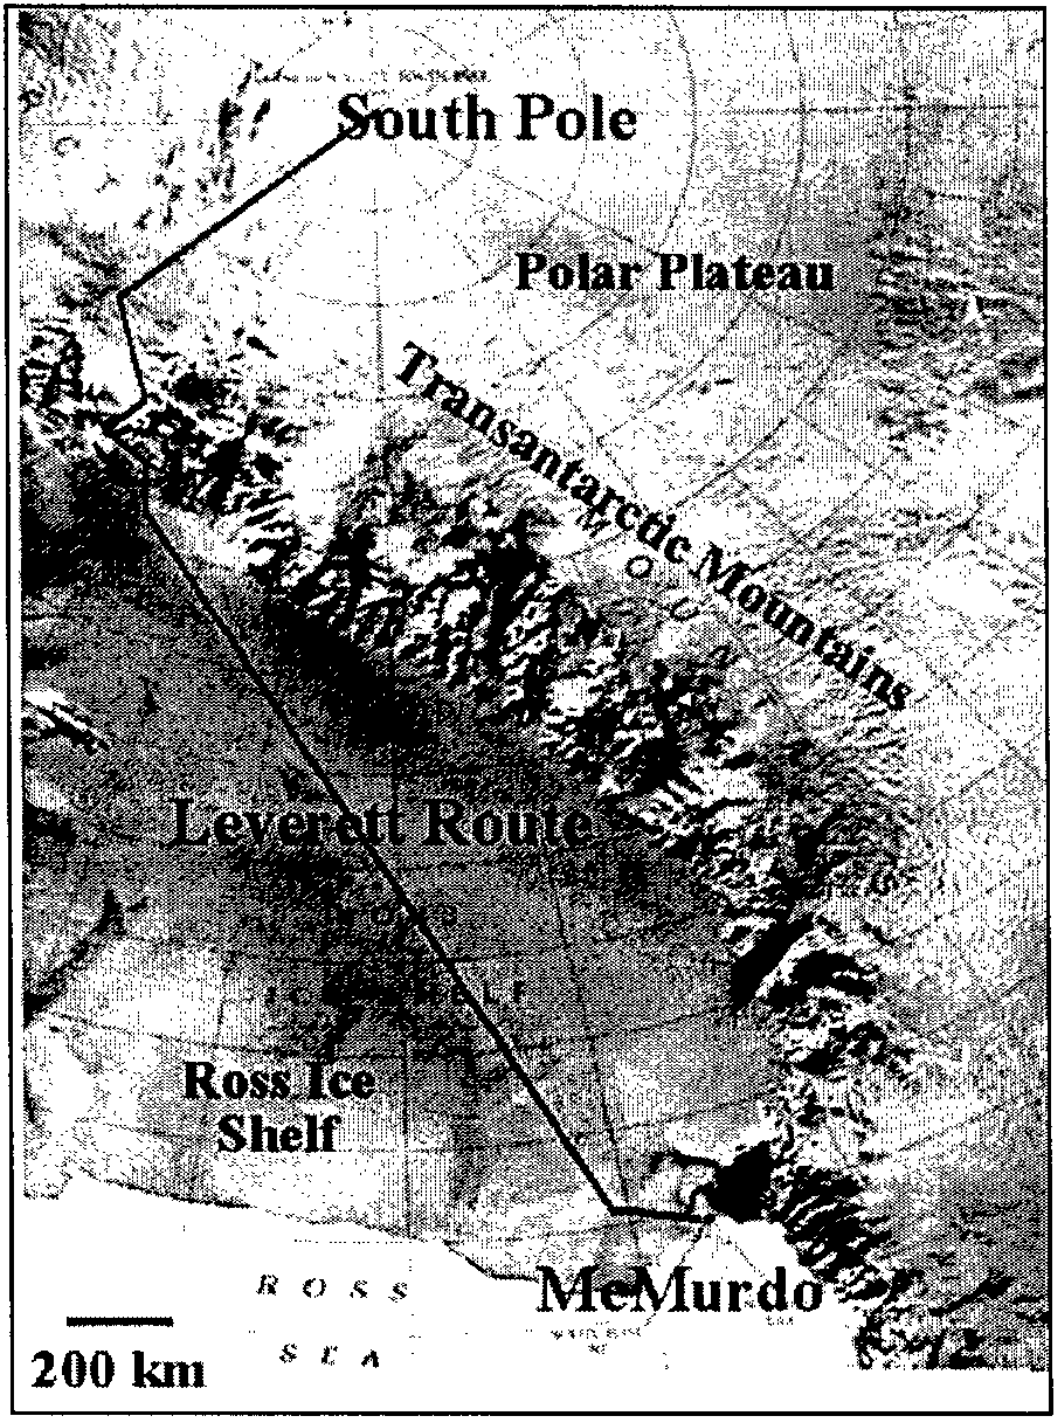
\includegraphics[width = 2in]{SPT_route}
    \caption{South Pole Traverse route from McMurdo Station across the McMurdo and Ross ice shelves, up the Leverett Glacier, and across the Polar Plateau to Amundsen-Scott South Pole Station. Reproduced from \cite{lever2004mobility}}
    \label{fig:SPT_route}
\end{figure}

SPT now operates two fleets of eight tractors, each operated by an eight-person crew.  Each fleet can deliver approximately 350,000 kg of payload per trip. This eliminates 30 air trips that were needed before to produce a net economic benefit of \$2M.  Logistics consume about 80\% of USAP's budget causing SPT productivity gains to have a 4:1 multiplier to increase the science budget. USAP has also expanded SPT's capability to support field science camps in West Antarctica and on the Ross Ice Shelf. The SPT fleets operate each day on 10 hour driving shifts, with an additional 2 hours devoted to maintenance and refueling.  Using this work schedule, a round trip to the South Pole requires approximately 50 days. In their present configuration, SPT completes 3 of these round trips per season. 

Automating the tractors to operate four manually and four as robotic followers would enable two driving shifts per day using the same eight-person crew. This would allow for additional trips per season per fleet, providing additional payload delivered via ground to the South Pole. Figure \ref{fig:tractor_convoy_image} shows five of the eight tractors used for the October 2015 South Pole journey. This highlights the potential for automation as vehicle pairs are offset at distances of approximately 100m in an unobstructed environment. An investment in automated tractors would have a large payoff in reducing the percentage of USAP's budget spent on logistics and could drastically increase science budgets. 
\begin{figure}[b]
    \centering
    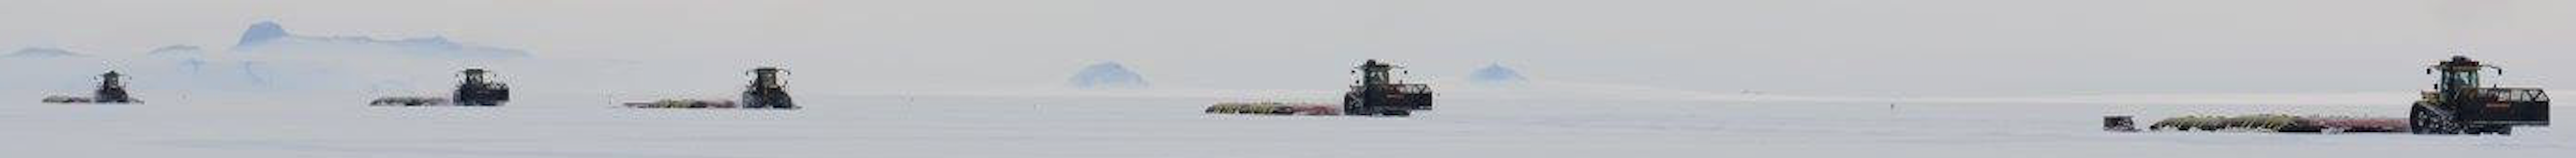
\includegraphics[width=6in]{tractor_convoy_image}
    \caption{Five of the eight tractors used for the October 2015 South Pole journey at the Ross Ice Shelf}
    \label{fig:tractor_convoy_image}
\end{figure}
However, maintaining mobility is the key to adhering to these proposed fast pace traverse schedules to ensure economic benefit from an initial investment.  High sled payloads increase payback but also increase risks of immobilization delays. In addition, terrain trafficability conditions vary substantially for SPT operations. This includes different snow conditions on a single trip along the route and variations between trips due to variations in seasonal temperature and its effect on the snow-terrain properties. Implementation of autonomous control modes for robotic follower tractors that address the large variations in mobility conditions would enable these fast pace traverses to produce the desired economic benefits.

\section{Scope of Work}
The objective of the work is to investigate and develop methods for heavy, off-road, tracked tractors to be autonomous while pulling a heavy payload. This task is challenging as the overall system dynamics have complex interacting nonlinearities along with temporal and spatial terrain uncertainties that can be difficult to estimate in real-time. The investigations presented and conclusions reached in this thesis are based on simulation results derived from physically motivated modeling approaches combined from the terramechanics and automotive literature. The modeling approaches used are validated for longitudinal motion from experimental data collected in Antarctica. This is sufficient as this is the main operating mode for tracked vehicles under load. The beginning chapters of the thesis will outline three different model derivations along with simulation results. These models are developed to address the following control modes for tractor autonomy where each successive one aims to handle a more challenging mobility condition:
\begin{enumerate}
    \item Leader-Follower Mode: This control mode will drive autonomous, follower tractors during the majority of traverse operations when there is sufficient traction to pull payloads. In this mode, unmanned tractors will use a manned leader as a reference utilizing knowledge of their position, speed, heading, and driver inputs of throttle and gear selection. An interchangeable name for this mode will be Control Mode 1.
    \item Traction Control Mode: This second control mode will be entered when the tractor has exceeded some track slip value that indicates the presence of a softer, lower traction terrain. The tractor will not be permitted to turn to maximize mobility due to the governing dynamics. The controllers developed in this mode will adjust gear and throttle inputs to regulate track slip and maximize traction. An interchangeable name for this mode will be Control Mode 2.
    \item Winch Control Mode: This third control mode is entered when the tractor has an indication that no combination of gear and throttle inputs in the Traction Control Mode will allow it to maintain mobility. The only available option is to use a towing winch and let out the payload to reduce the drawbar load on the tractor. If the softer, low traction terrain area is shorter than the cable length available from the winch, the winch can be used to reel the payload back in once firmer ground is reached. However, if there is insufficient cable length, this control mode will be the failure point for tractor mobility.
\end{enumerate}


Chapter \ref{ch:RSBD} derives a simplified single body model where the payload puts a constant load on the tractor in one direction. This simplified model is used in control modes 2 and 3 in order to compute estimates of tractor states, track forces, and terrain parameters. The second model derived in Ch. \ref{ch:RMBD} captures the complete vehicle dynamics that are present in SPT's current towing configuration by including the drawbar arm and sled in a multi-body model. This eliminates the assumption of constant one directional loading at the drawbar so that payload stability issues can be realized in numerical experiments. This model is used to develop and test the strategy for the Leader-Follower Mode. The third model derived in Ch. \ref{ch:RMBDW} is also a multi-body model but focuses only on longitudinal motion and includes a winch to explore its viability to help tractors maintain mobility in soft terrain. This model is used for numerical experiments to explore and prove viable strategies for control modes 2 and 3. These dynamics modeling chapters are self-enclosed with references listed for extended discussions. 

